\section{Auswertung}
\label{sec:Auswertung}
\subsection{Magnetische Flußdichte zweier Spulen}
 \begin{table}[H]
  \centering
    \begin{subtable}{.4\linewidth}
      \centering
        \csvreader[tabular=c|c,
  head=false, 
  table head= $x\:/\:\si{\centi\meter}$ & $B\:/\:\si{\milli\tesla}$ \\\midrule,
  late after line= \\]
  {LSpule.csv}{1=\eins, 2=\zwei}{$\num{\eins}$ & $\num{\zwei}$}
  \caption{lange Spule}
    \end{subtable} 
    \begin{subtable}{.4\linewidth}
      \centering
        %\caption{Messwerte x und y sowie das Ergebnis nach Gleichung blabla.}
      \csvreader[tabular=c|c,
  head=false, 
  table head= $x\:/\:\si{\centi\meter}$ & $B\:/\:\si{\milli\tesla}$ \\\midrule,
  late after line= \\]
  {KSpule.csv}{1=\eins, 2=\zwei}{$\num{\eins}$ & $\num{\zwei}$}
  
  \caption{Kurze Spule}
 
    \end{subtable} 
        \caption{Magnetische Flußdichte zweier Spulen entlang ihrer Symmetrieachsen}
    \label{tab:1}
\end{table}


\noindent Die Messwerte für die magnetische Flußdichte der 
langen und der kurzen Spule sind in Tabelle \ref{tab:1} aufgelistet.
Außerdem sind die Werte der langen Spule zusammen mit
dem Theoriewert, welcher sich nach Gleichung \ref{eq:a} als
\begin{equation}
  B_{L,t}=1,909\,\si{\milli\tesla}\nonumber
\end{equation}
berechnen lässt, in Abbildung \ref{fig:a} in einem
xB-Diagramm aufgetragen, wobei der Nullpunkt
von x am Anfang der Spule liegt. Bei der Berechung wurde $\mu_0=4 \cdot \pi \cdot 10^{-7}$ nach \cite{sample} angenommen.

\begin{figure}[H]
\centering
  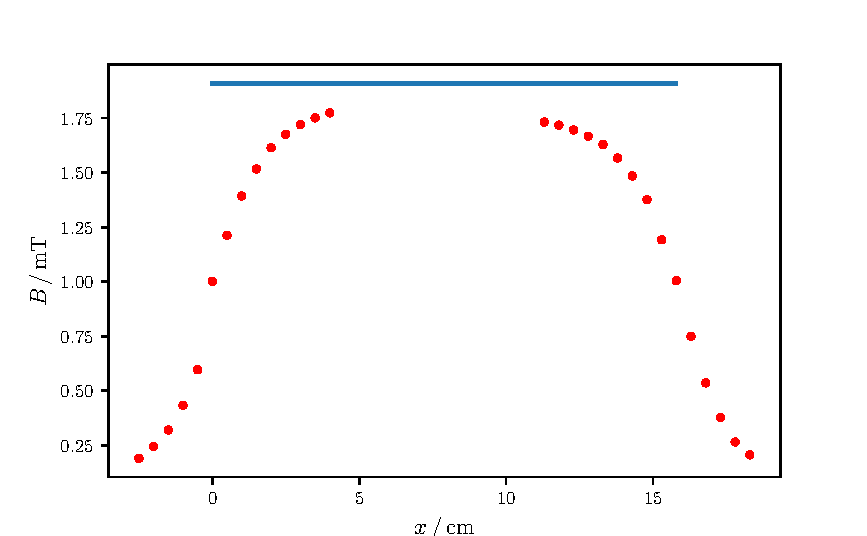
\includegraphics[width=9cm]{plot1-1.pdf}
  \caption{Flussdichte $B$ entlang der Symmetrieachse einer langen Spule}
  \label{fig:a}
\end{figure}
\noindent Beim Vergleich mit der Theorie fällt auf, dass
die gemessenen Werte noch in der Spule am Randbereich
abfallen und auch in der Mitte nicht ganz den vollen
Theoriewert erreichen.


\noindent Die Messwerte der kurzen Spule sind in Abbildung
\ref{fig:b} als xB-Diagramm dargestellt.

\begin{figure}
\centering
  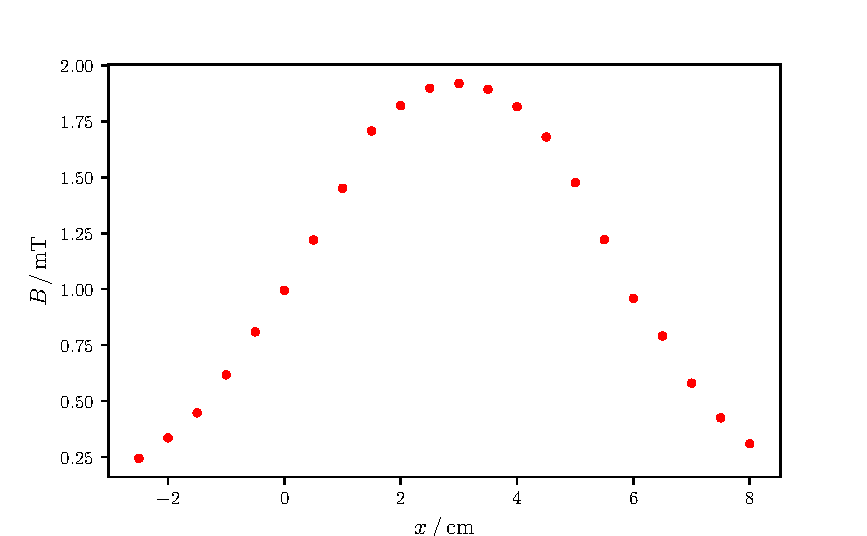
\includegraphics[width=9cm]{plot1-2.pdf}
   \caption{Flussdichte $B$ entlang der Symmetrieachse einer kurzen Spule}
  \label{fig:b}
\end{figure}

\subsection{Magnetische Flußdichte eines Helmholzspulenpaares}
  
  \begin{table}[H]
  \centering
    \begin{subtable}{.3\linewidth}
      \centering
        \csvreader[tabular=c|c,
    head=false, 
    table head= $x\:/\:\si{\centi\meter}$ & $B\:/\:\si{\milli\tesla}$ \\\midrule,
    late after line= \\]
    {Messung1.csv}{1=\eins, 2=\zwei}{$\num{\eins}$ & $\num{\zwei}$}
            \caption{Abstand $l=10\:\:\si{\centi\meter}$}

    \end{subtable}%
    \begin{subtable}{.3\linewidth}
      \centering
        \csvreader[tabular=c|c,
    head=false, 
    table head= $x\:/\:\si{\centi\meter}$ & $B\:/\:\si{\milli\tesla}$ \\\midrule,
    late after line= \\]
    {Messung2.csv}{1=\eins, 2=\zwei}{$\num{\eins}$ & $\num{\zwei}$}
            \caption{Abstand $l=14\:\:\si{\centi\meter}$}

    \end{subtable} 
    \begin{subtable}{.3\linewidth}
      \centering
        %\caption{Messwerte x und y sowie das Ergebnis nach Gleichung blabla.}
    \csvreader[tabular=c|c,
    head=false, 
    table head= $x\:/\:\si{\centi\meter}$ & $B\:/\:\si{\milli\tesla}$ \\\midrule,
    late after line= \\]
    {Messung3.csv}{1=\eins, 2=\zwei}{$\num{\eins}$ & $\num{\zwei}$}
            \caption{Abstand $l=17\:\:\si{\centi\meter}$}

    \end{subtable} 
        \caption{Flussdichte $B$ auf der Symmetrieachse eines Helmholtzspulennpaares}
    \label{tab:3}
\end{table}
Für die drei unterschiedlichen Abstände der Helmholtzspulen
ergeben sich die Messwerte in Tabelle \ref{tab:3}. 
\begin{figure}[H]
\centering

  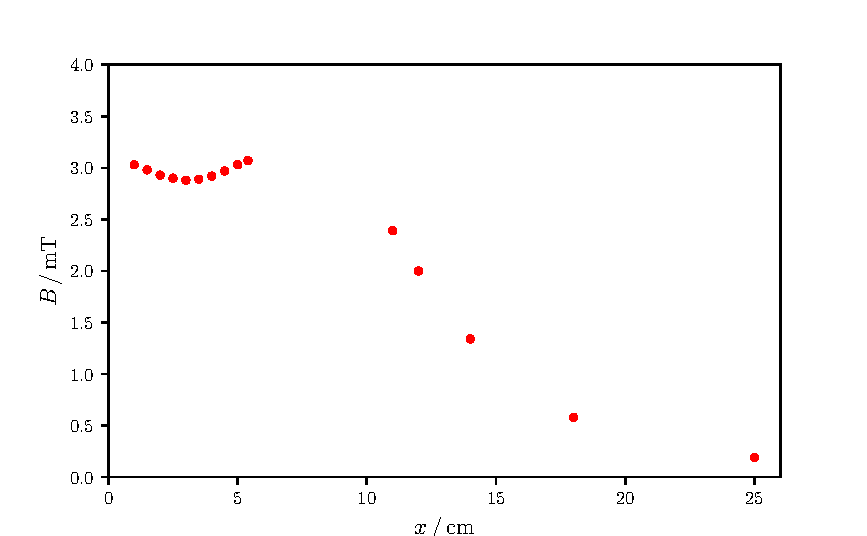
\includegraphics[width=9cm]{plot2-1.pdf}
  \caption{Flussdichte $B$ auf der Symmetrieachse eines Helmholtzspulenpaares mit Abstand $l=10\:\:\si{\centi\meter}$}
\end{figure}
\noindent Der Theoriewert der magnetischen Flußdichte im Mittelpunkt
beim Abstand von 10\,cm kann kann mit Gleichung \ref{eq:b}
als
  \begin{equation}
    B=2,87\,\si{\milli\tesla}\nonumber
  \end{equation}
\noindent ermittelt werden. Er kann mit dem Messwert 
\begin{equation}
    B=2,88\,\si{\milli\tesla}\nonumber
  \end{equation}
\noindent verglichen werden. 
\begin{figure}[H]
\centering
  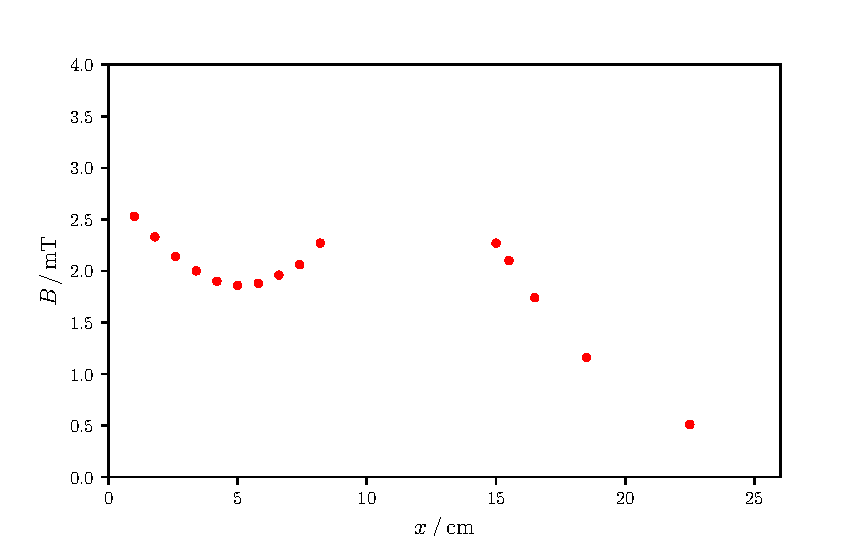
\includegraphics[width=9cm]{plot2-2.pdf}
    \caption{Flussdichte $B$ auf der Symmetrieachse eines Helmholtzspulenpaares mit Abstand $l=14\:\:\si{\centi\meter}$}

\end{figure}
\noindent Für einen Abstand von 14\,cm kann die magnetische
Flussdichte im Mittelpunkt über Gleichung \ref{eq:b}
als
  \begin{equation}
    B=1,782\,\si{\milli\tesla}\nonumber
  \end{equation}
\noindent berechnet werden und mit dem Messwert  
\begin{equation}
    B= 1,883\,\si{\milli\tesla}\nonumber
  \end{equation}
\noindent verglichen werden. 
\begin{figure}[H]
\centering
  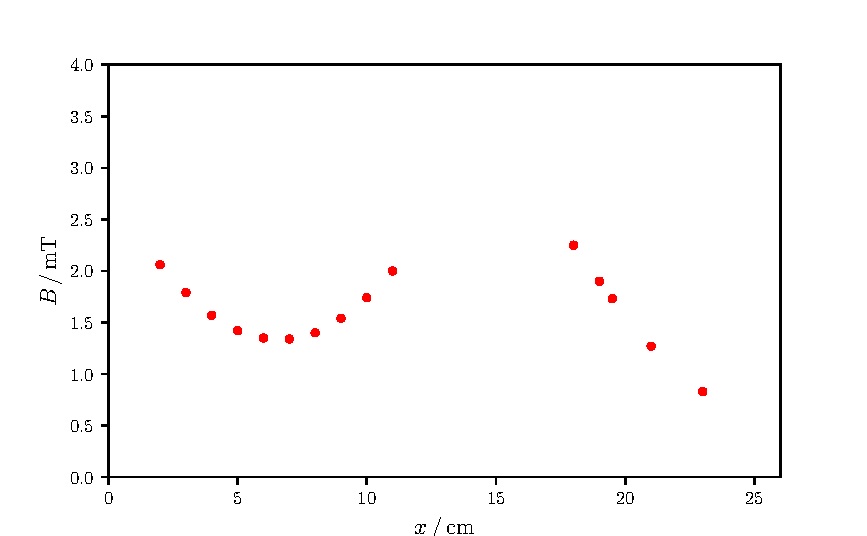
\includegraphics[width=9cm]{plot2-3.pdf}
    \caption{Flussdichte $B$ auf der Symmetrieachse eines Helmholtzspulenpaares mit Abstand $l=17\:\:\si{\centi\meter}$}
\end{figure}
\noindent Bei einem Abstand von 17\,cm ergibt sich
der Theoriewert der magnetischen Flussdichte mit
Gleichung \ref{eq:b} als
  \begin{equation}
    B=1,254\,\si{\milli\tesla}\nonumber
  \end{equation}
\noindent Er kann mit dem Messwert 
\begin{equation}
    B=1,338\,\si{\milli\tesla}\nonumber
  \end{equation}
\noindent verglichen werden. 

Es fällt auf, dass alle Messwerte, besonders der erste,
nahe am errechneten Theoriewert liegen.


\subsection{Hysteresekurve einer Spule mit Eisenkern}

  \begin{table}[H]
  \centering
  
    \begin{subtable}{.33\linewidth}
      \centering
      \small
        \csvreader[tabular=c|c|c,
  head=false, 
  table head= $I\:/\:\si{\ampere}$ & $B\:/\:\si{\milli\tesla}$ & $H \:/\: \si{\ampere\cdot\m^{-1}}$ \\\midrule,
  late after line= \\]
  {Neukurve.csv}{1=\eins, 2=\zwei, 3=\drei}{$\num{\eins}$ & $\num{\zwei}$ & $\num{\drei}$}
  \caption{Neukurve}
    \end{subtable}%
    \begin{subtable}{.33\linewidth}
      \centering
      \small
        \csvreader[tabular=c|c|c,
  head=false, 
  table head= $I\:/\:\si{\ampere}$ & $B\:/\:\si{\milli\tesla}$ & $H \:/\: \si{\ampere\cdot\m^{-1}}$ \\\midrule,
  late after line= \\]
  {tief.csv}{1=\eins, 2=\zwei, 3=\drei}{$\num{\eins}$ & $\num{\zwei}$ & $\num{\drei}$}
  \caption{Verringern des äußeren Magnetfeldes}
    \end{subtable} 
    \begin{subtable}{.33\linewidth}
      \centering
      \small
        %\caption{Messwerte x und y sowie das Ergebnis nach Gleichung blabla.}
        \csvreader[tabular=c|c|c,
  head=false, 
  table head= $I\:/\:\si{\ampere}$ & $B\:/\:\si{\milli\tesla}$ & $H \:/\: \si{\ampere\cdot\m^{-1}}$ \\\midrule,
  late after line= \\]
  {hoch.csv}{1=\eins, 2=\zwei, 3=\drei}{$\num{\eins}$ & $\num{\zwei}$ & $\num{\drei}$}
  \caption{Erhöhen des äußeren Magnetfeldes}
    \end{subtable} 
        \caption{Magnetische Feldstärke $B$ in Abhängigkeit der magnetischen Feldstärke $H$}
    \label{tab:4}
\end{table}

Die Tabelle \ref{tab:4} beinhaltet die Messwerte für
die Spule mit Eisenkern. Dabei ist die Stromrichtung
durch ein Vorzeichen bei der Stromstärke angegeben. Aus
den Messwerten lässt sich sofort der Wert für die
Sättigungsmagnetisierung 
\begin{equation}
  B_S=732\,\si{\milli\tesla}\nonumber
\end{equation}
\noindent und der Wert für die Remanenz
\begin{equation}
  B_r=131\,\si{\milli\tesla}\nonumber
\end{equation}
\noindent ablesen.

Um die Koerzitivkraft $H_c$ zu bestimmen muss jedoch
zunächst eine Ausgleichsgerade um den Achsennullpunkt
erstellt werden um die magnetische Erregung bei
$B=0\,\si{\milli\tesla}$ zu erhalten. Dies wurde hier
mit matplotlib \cite{matplotlib} umgesetzt und ist in Abbildung \ref{fig:ZZZ}zu sehen. 

Mit dieser Methode ergibt sich die Koerzitivkraft als
\begin{equation}
  H_c=463\,\si{\ampere\cdot\meter^{-1}}\nonumber.
\end{equation}

\begin{figure}
  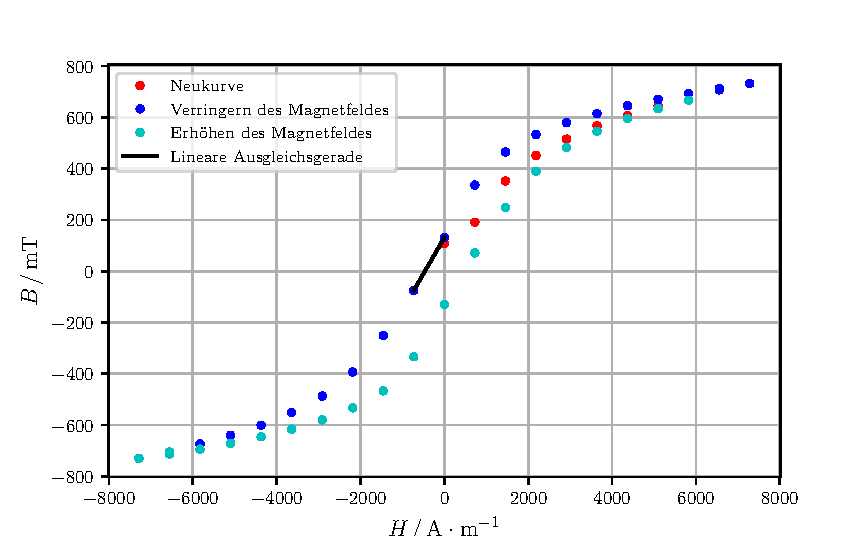
\includegraphics{plot3.pdf}
  \caption{ZZZ}
\end{figure}


